\documentclass{standalone}
\usepackage{tikz}
\usepackage{tikz-qtree}
\usetikzlibrary{positioning}
\definecolor{indianred}{RGB}{205,92,92}

\begin{document}
    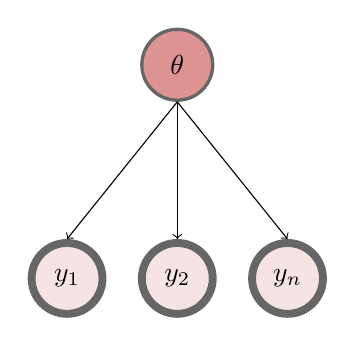
\begin{tikzpicture}[
        roundnode/.style={circle, draw=black!60, very thick, minimum size=9mm}]
        \node[roundnode,draw=none] (poolparams) {};
        \node[roundnode,draw=none] (localtwo) [below=0.4cm of poolparams] {};
        \node[roundnode,fill=indianred!66] (poolparams) {$\theta$};
        \node[roundnode,fill=indianred!17,  line width=1mm] (y2) [below=0.4cm of localtwo] {$y_{2}$};
        \node[roundnode,fill=indianred!17,line width=1mm] (y1) [left=0.4cm of y2] {$y_{1}$};
        \node[roundnode,fill=indianred!17,line width=1mm] (yn) [right=0.4cm of y2] {$y_{n}$};
        \draw[->] (poolparams.south) -- (y1.north);
        \draw[->] (poolparams.south) -- (y2.north);
        \draw[->] (poolparams.south) -- (yn.north);
\end{tikzpicture}\hspace{0.5cm}
    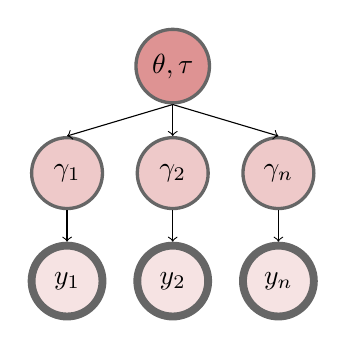
\begin{tikzpicture}[
        roundnode/.style={circle, draw=black!60, very thick, minimum size=9mm}]
        \node[roundnode,fill=indianred!66] (poolparams) {$\theta, \tau$};
        \node[roundnode,fill=indianred!33] (localtwo) [below=0.4cm of poolparams] {$\gamma_{2}$};
        \node[roundnode,fill=indianred!33] (localone) [left=0.4cm of localtwo] {$\gamma_{1}$};
        \node[roundnode,fill=indianred!33] (localn) [right=0.4cm of localtwo] {$\gamma_{n}$};
        \node[roundnode,fill=indianred!17,  line width=1mm] (y2) [below=0.4cm of localtwo] {$y_{2}$};
        \node[roundnode,fill=indianred!17,  line width=1mm] (y1) [below=0.4cm of localone] {$y_{1}$};
        \node[roundnode,fill=indianred!17,  line width=1mm] (yn) [below=0.4cm of localn] {$y_{n}$};
        \draw[->] (poolparams.south) -- (localone.north);
        \draw[->] (poolparams.south) -- (localtwo.north);
        \draw[->] (poolparams.south) -- (localn.north);
        \draw[->] (localone.south) -- (y1.north);
        \draw[->] (localtwo.south) -- (y2.north);
        \draw[->] (localn.south) -- (yn.north);
\end{tikzpicture}\hspace{0.5cm}
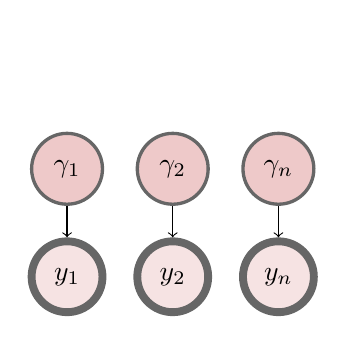
\begin{tikzpicture}[
        roundnode/.style={circle, draw=black!60, very thick, minimum size=9mm}]
        \node[roundnode, draw=none, fill=red!0] (poolparams) {};
        \node[roundnode,fill=indianred!33] (localtwo) [below=0.4cm of poolparams] {$\gamma_{2}$};
        \node[roundnode,fill=indianred!33] (localone) [left=0.4cm of localtwo] {$\gamma_{1}$};
        \node[roundnode,fill=indianred!33] (localn) [right=0.4cm of localtwo] {$\gamma_{n}$};
        \node[roundnode,fill=indianred!17,  line width=1mm] (y2) [below=0.4cm of localtwo] {$y_{2}$};
        \node[roundnode,fill=indianred!17,  line width=1mm] (y1) [below=0.4cm of localone] {$y_{1}$};
        \node[roundnode,fill=indianred!17,  line width=1mm] (yn) [below=0.4cm of localn] {$y_{n}$};
        \draw[->] (localone.south) -- (y1.north);
        \draw[->] (localtwo.south) -- (y2.north);
        \draw[->] (localn.south) -- (yn.north);
\end{tikzpicture}
\end{document}
    
